\chapter{Simplex Initialization}
In the previous chapter, we introduced the Simplex Algorithm and showed how to manipulate the $\mathbf{A}$, $\mathbf{B}$ and $\mathbf{N}$ matrices as we execute it. In this chapter, we will discuss the issue of finding an initial basic feasible solution to start execution of the Simplex Algorithm. 

\section{Artificial Variables}
So far we have investigated linear programming problems that had form:
\begin{displaymath}
\begin{aligned}
\max\;\; & \mathbf{c}^T\mathbf{x}\\
s.t.\;\; & \mathbf{A}\mathbf{x} \leq \mathbf{b}\\
& \mathbf{x} \geq \mathbf{0}
\end{aligned}
\end{displaymath}
In this case, we use slack variables to convert the problem to:
\begin{displaymath}
\begin{aligned}
\max\;\; & \mathbf{c}^T\mathbf{x}\\
s.t.\;\; & \mathbf{A}\mathbf{x} + \mathbf{I}_m \mathbf{x_s}  = \mathbf{b}\\
& \mathbf{x},\mathbf{x_s} \geq \mathbf{0}
\end{aligned}
\end{displaymath}
where $\mathbf{x_s}$ are slack variables, one for each constraint. If $\mathbf{b} \geq \mathbf{0}$, then our initial basic feasible solution can be $\mathbf{x} = \mathbf{0}$ and $\mathbf{x_s} = \mathbf{b}$ (that is, our initial basis matrix is $\mathbf{B} = \mathbf{I}_m$). We have also explored small problems where a graphical technique could be used to identify an initial extreme point of a polyhedral set and thus an initial basic feasible solution for the problem.

Suppose now we wish to investigate problems in which we do not have a problem structure that lends itself to easily identifying an initial basic feasible solution. The simplex algorithm requires an initial BFS to begin execution and so we must develop a method for finding such a BFS. 

For the remainder of this chapter we will assume, unless told otherwise, that we are interested in solving a linear programming problem provided in Standard Form. That is:
\begin{equation}
P\left\{
\begin{aligned}
\max\;\; & \mathbf{c}^T\mathbf{x}\\
s.t.\;\; & \mathbf{A}\mathbf{x} = \mathbf{b}\\
& \mathbf{x} \geq \mathbf{0}
\end{aligned}\right.
\end{equation}
and that $\mathbf{b} \geq \mathbf{0}$. Clearly our work in Chapter 3 shows that any linear programming problem can be put in this form. 

Suppose to each constraint $\mathbf{A}_{i\cdot}\mathbf{x} = \mathbf{b}_i$ we associate an \textit{artificial variable} ${x_{a_i}}$. We can replace constraint $i$ with:
\begin{equation}
\mathbf{A}_{i\cdot}\mathbf{x} + {x_{a_i}} = \mathbf{b}_i
\label{eqn:ModifiedConstraint}
\end{equation}
Since $\mathbf{b}_i \geq 0$, we will require $x_{a_i} \geq 0$. If ${x_{a_i}} = 0$, then this is simply the original constraint. Thus if we can find values for the ordinary decision variables $\mathbf{x}$ so that $x_{a_i}=0$, then constraint $i$ is satisfied. If we can identify values for $\mathbf{x}$ so that all the artificial variables are zero and $m$ variables of $\mathbf{x}$ are non-zero, then the modified constraints described by Equation \ref{eqn:ModifiedConstraint} are satisfied and we have identified an initial basic feasible solution. 

Obviously, we would like to penalize non-zero artificial variables. This can be done by writing a new linear programming problem:
\begin{equation}
P_1\left\{
\begin{aligned}
\min\;\; & \mathbf{e}^T\mathbf{x_a}\\
s.t.\;\; & \mathbf{A}\mathbf{x} + \mathbf{I}_m\mathbf{x_a} = \mathbf{b}\\
& \mathbf{x},\mathbf{x_a} \geq \mathbf{0}
\end{aligned}\right.
\end{equation}

\begin{remark} We can see that the artificial variables are similar to slack variables, but they should have zero value because they have no true meaning in the original problem $P$. They are introduced \textit{artificially} to help identify an initial basic feasible solution to Problem $P$. 
\end{remark}

\begin{lemma} The optimal objective function value in Problem $P_1$ is bounded below by $0$. Furthermore, if the optimal solution to problem $P_1$ has $\mathbf{x_a} = \mathbf{0}$, then the values of $\mathbf{x}$ form a feasible solution to Problem $P$. 
\label{lem:PhaseILem}
\end{lemma}

\begin{proof} Clearly, setting $\mathbf{x_a}= \mathbf{0}$ will produce an objective function value of zero. Since $\mathbf{e} > \mathbf{0}$, we cannot obtain a smaller objective function value. If at optimality we have $\mathbf{x_a} = \mathbf{0}$, then we know that $m$ of the variables in $\mathbf{x}$ are in the basis and the remaining variables (in both $\mathbf{x}$ and $\mathbf{x_a}$) are not in the basis and hence at zero. Thus we have found a basic feasible solution to Problem $P$. 
\end{proof}

\begin{example} Consider the following problem:
\begin{equation}
\begin{aligned}
\min\;\; & 	x_1 + 2x_2\\
s.t.\;\; &	x_1 + 2x_2 \geq 12\\
		 &	2x_1 + 3x_2 \geq 20\\
		 &	x_1, x_2 \geq 0
\end{aligned}
\end{equation}
We can convert the problem to standard form by adding two surplus variables:
\begin{equation}
\begin{aligned}
\min\;\; & 	x_1 + 2x_2\\
s.t.\;\; &	x_1 + 2x_2 - s_1  = 12\\
		 &	2x_1 + 3x_2 - s_2 = 20\\
		 &	x_1, x_2, s_1, s_2 \geq 0
\end{aligned}
\end{equation}
It's not clear what a good basic feasible solution would be for this. Clearly, we cannot set $x_1 = x_2 = 0$ because we would have $s_1 = -12$ and $s_2 = -20$, which is not feasible. We can introduce two artificial variables ($x_{a_1}$ and $x_{a_2}$) and create a new problem $P_1$. 
\begin{equation}
\begin{aligned}
\min\;\; & 	x_{a_1} + x_{a_2}\\
s.t.\;\; &	x_1 + 2x_2 - s_1  + x_{a_1} = 12\\
		 &	2x_1 + 3x_2 - s_2 + x_{a_2} = 20\\
		 &	x_1, x_2, s_1, s_2,x_{a_1},x_{a_2} \geq 0
\end{aligned}
\end{equation}
A basic feasible solution for our \textit{artificial problem} would let $x_{a_1} = 12$ and $x_{a_2} = 20$. The pertinent matrices in this case are:
\begin{displaymath}
\mathbf{A} = \begin{bmatrix}
1 & 2 & -1 & 0 & 1 & 0\\
2 & 3 & 0 & -1 & 0 & 1
\end{bmatrix}\;\;\;\;
\mathbf{b} = \begin{bmatrix}
12\\20
\end{bmatrix}
\end{displaymath}
\begin{displaymath}
\mathbf{B} = \begin{bmatrix}
1 & 0\\
0 & 1
\end{bmatrix}\;\;\;\;
\mathbf{N} = \begin{bmatrix}
1 & 2 & -1 & 0\\
2 & 3 & 0 & -1
\end{bmatrix}\;\;\;\;
\mathbf{B}^{-1}\mathbf{b} = 
\begin{bmatrix}
12\\20
\end{bmatrix}
\end{displaymath}
\begin{displaymath}
\mathbf{c_B} = \begin{bmatrix}
1\\
1
\end{bmatrix}\;\;\;\;
\mathbf{c_N} = \begin{bmatrix}
0\\0\\0\\0
\end{bmatrix}
\end{displaymath}
\begin{displaymath}
\mathbf{c}_\mathbf{B}^TB^{-1}\mathbf{b} = 32\;\;\;\;
\mathbf{c}_\mathbf{B}^T\mathbf{B}^{-1}\mathbf{N} - \mathbf{c}_{\mathbf{N}}^T = \begin{bmatrix}
3 & 5 & -1 & -1
\end{bmatrix}
\end{displaymath}
We can construct an initial tableau for this problem as:
\begin{equation}
\begin{array}{c}
\\
z\\
x_{a_1}\\
x_{a_2}
\end{array}
\left[
\begin{array}{c|cccccc|c}
z & x_1 & x_2 & s_1 & s_2 & x_{a_1} & x_{a_2} & \text{RHS}\\
\hline
1 & 3 & 5 & -1 & -1 & 0 & 0 & 32\\
\hline
0 & 1 & 2 & -1 & 0  & 1 & 0 & 12\\
0 & 2 & 3 & 0  & -1 & 0 & 1 & 20
\end{array}
\right]
\end{equation}
This is a minimization problem, so if $z_j - c_j > 0$, then entering $x_j$ will improve (decrease) the objective value because $\partial z/\partial x_j < 0$. In this case, we could enter either $x_1$ or $x_2$ to improve the objective value. Let's assume we enter variable $x_1$. Performing the minimum ratio test we see:
\begin{equation}
\begin{array}{c}
\\
z\\
x_{a_1}\\
x_{a_2}
\end{array}
\left[
\begin{array}{c|cccccc|c}
z & x_1 & x_2 & s_1 & s_2 & x_{a_1} & x_{a_2} & \text{RHS}\\
\hline
1 & 3 & 5 & -1 & -1 & 0 & 0 & 32\\
\hline
0 & 1 & 2 & -1 & 0  & 1 & 0 & 12\\
0 & \fbox{2} & 3 & 0  & -1 & 0 & 1 & 20
\end{array}
\right]
\begin{array}{c}
\text{MRT}(x_1)\\
\hline
\\
12\\
20/2 = 10
\end{array}
\end{equation}
Thus $x_{a_2}$ leaves the basis and $x_1$ enters. The new tableau becomes:
\begin{equation}
\begin{array}{c}
\\
z\\
x_{a_1}\\
x_{1}
\end{array}
\left[
\begin{array}{c|cccccc|c}
z & x_1 & x_2 & s_1 & s_2 & x_{a_1} & x_{a_2} & \text{RHS}\\
\hline
1 & 0 & 1/2 & -1 & 1/2 & 0 & -3/2 & 2\\
\hline
0 & 0 & 1/2 & -1 & 1/2  & 1 & -1/2 & 2\\
0 & 1 & 3/2 & 0  & -1/2 & 0 & 1/2 & 10
\end{array}
\right]
\end{equation}
In this case, we see that $x_2$ should enter the basis. Performing the minimum ratio test, we obtain:
\begin{equation}
\begin{array}{c}
\\
z\\
x_{a_1}\\
x_{1}
\end{array}
\left[
\begin{array}{c|cccccc|c}
z & x_1 & x_2 & s_1 & s_2 & x_{a_1} & x_{a_2} & \text{RHS}\\
\hline
1 & 0 & 1/2 & -1 & 1/2 & 0 & -3/2 & 2\\
\hline
0 & 0 & \fbox{1/2} & -1 & 1/2  & 1 & -1/2 & 2\\
0 & 1 & 3/2 & 0  & -1/2 & 0 & 1/2 & 10
\end{array}
\right]
\begin{array}{c}
\text{MRT}(x_2)\\
\hline
\\
4\\
20/3
\end{array}
\end{equation}
Thus we see that $x_{a_2}$ leaves the basis and we obtain:
\begin{equation}
\begin{array}{c}
\\
z\\
x_{2}\\
x_{1}
\end{array}
\left[
\begin{array}{c|cccccc|c}
z & x_1 & x_2 & s_1 & s_2 & x_{a_1} & x_{a_2} & \text{RHS}\\
\hline
1 & 0 & 0 & 0 & 0 & -1 & -1 & 0\\
\hline
0 & 0 & 1 & -2 & 1  & 2 & -1 & 4\\
0 & 1 & 0 & 3  & -2 & -3 & 2 & 4
\end{array}
\right]
\label{eqn:LastPhase1Tableau}
\end{equation}
At this point, we have eliminated both artificial variables from the basis and we have identified and initial basic feasible solution to the original problem: $x_1 = 4$, $x_2 = 4$, $s_1 = 0$ and $s_2 = 0$. The process of moving to a feasible solution in the original problem is shown in Figure \ref{fig:PhaseISimplex}.
\begin{figure}[htbp]
\centering
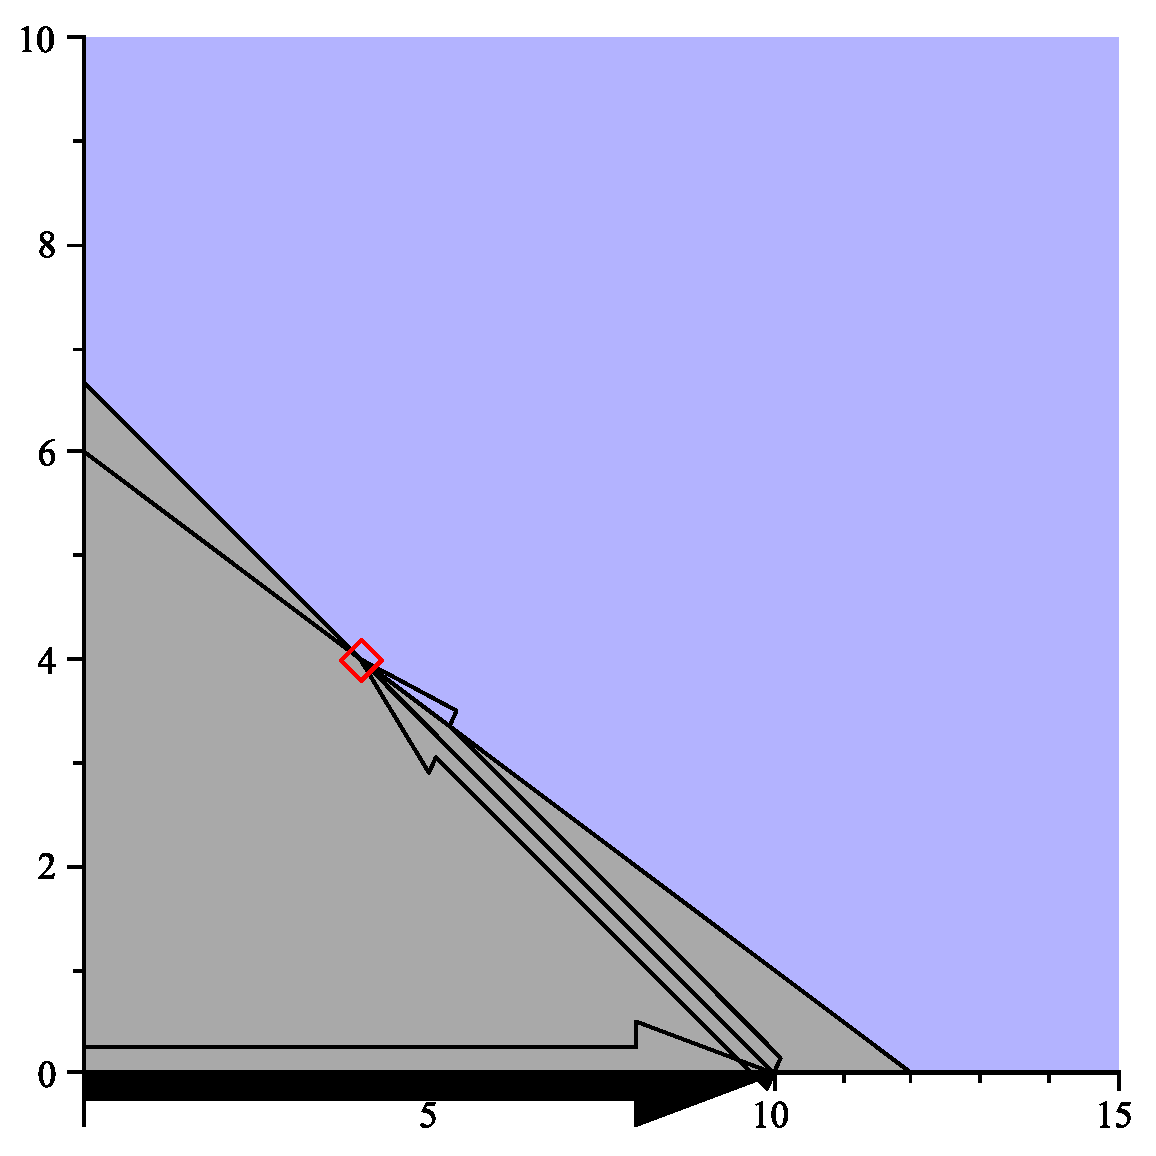
\includegraphics[scale=0.35]{PhaseISimplex.pdf}
\caption{Finding an initial feasible point: Artificial variables are introduced into the problem. These variables allow us to move through non-feasible space. Once we reach a feasible extreme point, the process of optimizing Problem $P_1$ stops.}
\label{fig:PhaseISimplex}
\end{figure}
\label{ex:ArtificialVariables}

We could now continue on to solve the initial problem we were given. At this point, our basic feasible solution makes $x_2$ and $x_1$ basic variables and $s_1$ and $s_2$ non-basic variables. Our problem data are:
\begin{displaymath}
\mathbf{x}_\mathbf{B} = \begin{bmatrix}x_2 \\ x_1\end{bmatrix}\quad
\mathbf{x}_\mathbf{N} = \begin{bmatrix}s_1 \\ s_2\end{bmatrix}
\end{displaymath}
Note that we keep the basic variables in the order in which we find them at the end of the solution to our first problem.  
\begin{displaymath}
\mathbf{A} = \begin{bmatrix}
1 & 2 & -1 & 0 \\
2 & 3 & 0 & -1
\end{bmatrix}\;\;\;\;
\mathbf{b} = \begin{bmatrix}
12\\20
\end{bmatrix}
\end{displaymath}
\begin{displaymath}
\mathbf{B} = \begin{bmatrix}
2 & 1\\
3 & 2
\end{bmatrix}\;\;\;\;
\mathbf{N} = \begin{bmatrix}
-1 & 0\\
 0 & -1
\end{bmatrix}\;\;\;\;
\mathbf{B}^{-1}\mathbf{b} = 
\begin{bmatrix}
4\\4
\end{bmatrix}
\end{displaymath}
\begin{displaymath}
\mathbf{c_B} = \begin{bmatrix}
2\\
1
\end{bmatrix}\;\;\;\;
\mathbf{c_N} = \begin{bmatrix}
0\\0
\end{bmatrix}
\end{displaymath}
\begin{displaymath}
\mathbf{c}_\mathbf{B}^TB^{-1}\mathbf{b} = 12\;\;\;\;
\mathbf{c}_\mathbf{B}^T\mathbf{B}^{-1}\mathbf{N} - \mathbf{c}_{\mathbf{N}}^T = \begin{bmatrix}
-1 & 0
\end{bmatrix}
\end{displaymath}

\textit{Notice that we don't have to do a lot of work to get this information out of the last tableau in Expression \ref{eqn:LastPhase1Tableau}.} The matrix $\mathbf{B}^{-1}$ is actually positioned in the columns below the artificial variables. This is because we started with an identity matrix in this position. As always, the remainder of the matrix holds $\mathbf{B}^{-1}\mathbf{N}$. Thus, we can read this final tableau as:

\begin{equation}
\begin{array}{c}
\\
z\\
x_{2}\\
x_{1}
\end{array}
\left[
\begin{array}{c|ccc|c}
z & \mathbf{x}_\mathbf{B} & \mathbf{s} & \mathbf{x}_a & \text{RHS}\\
\hline
1 & \mathbf{0} & \mathbf{0} & -\mathbf{e} & 0\\
\hline
\mathbf{0} & \mathbf{I}_2 & \mathbf{B}^{-1}\mathbf{N}  & \mathbf{B}^{-1} & \mathbf{B}^{-1}\mathbf{b}
\end{array}
\right]
\label{eqn:LastPhase1TableauX}
\end{equation}
In our case from Expression \ref{eqn:LastPhase1Tableau} we have:
\begin{equation}
\begin{array}{c}
\\
z\\
x_{2}\\
x_{1}
\end{array}
\left[
\begin{array}{c|cc|cc|cc|c}
z & x_1 & x_2 & s_1 & s_2 & x_{a_1} & x_{a_2} & \text{RHS}\\
\hline
1 & 0 & 0 & 0 & 0 & -1 & -1 & 0\\
\hline
0 & 0 & 1 & -2 & 1  & 2 & -1 & 4\\
0 & 1 & 0 & 3  & -2 & -3 & 2 & 4\\
\hline
- & \multicolumn{2}{c}{\mathbf{I}_2} & \multicolumn{2}{c}{\mathbf{B}^{-1}\mathbf{N}} & \multicolumn{2}{c}{\mathbf{B}^{-1}} & \mathbf{B}^{-1}\mathbf{b}
\end{array}
\right]
%\label{eqn:LastPhase1Tableau}
\end{equation}

We can use this information (and the reduced costs and objective function we computed) to start our tableau to solve the problem with which we began. Our next initial tableau will be:
\begin{equation}
\begin{array}{c}
\\
z\\
x_{2}\\
x_{1}
\end{array}
\left[
\begin{array}{c|cccc|c}
z & x_1 & x_2 & s_1 & s_2  & \text{RHS}\\
\hline
1 & 0 & 0 & -1 & 0 & 12\\
\hline
0 & 0 & 1 & -2 & 1  & 4\\
0 & 1 & 0 & 3  & -2 & 4
\end{array}
\right]
%\label{eqn:LastPhase1Tableau}
\end{equation}

Notice all we've done is removed the artificial variables from the problem and substituted the newly computed reduced costs for $s_1$ and $s_2$ ($-1$ and $0$) into Row 0 of the tableau. We've also put the correct objective function value ($12$) into Row 0 of the right hand side. We're now ready to solve the original problem. However, since this is a \textit{minimization problem} we can see we're already at a point of optimality. Notice that all reduced costs are either negative or zero, suggesting that entering any non-basic variable will at best keep the objective function value the same and at worst make the objective function worse. Thus we conclude that an optimal solution for our original problem is $x^*_1 = x^*_2 = 4$ and $s^*_1 = s^*_2 = 0$.
\end{example}

\begin{theorem} Let $\mathbf{x}^*,\mathbf{x_a}^*$ be an optimal feasible solution to problem $P_1$. Problem $P$ is feasible if and only if $\mathbf{x_a}^*=\mathbf{0}$.
\end{theorem}
\begin{proof} We have already proved in Lemma \ref{lem:PhaseILem} that if $\mathbf{x_a}^*=\mathbf{0}$, then $\mathbf{x}^*$ is a feasible solution to $P$ and thus $P$ is feasible. 

Conversely, suppose that $P$ is feasible. Then $P$ has at least one basic feasible solution because the feasible region of $P$ is a polyhedral set and we are assured by Lemma \ref{lem:FiniteExtremePoints} that this set has at least one extreme point. Now we can simply let $\mathbf{x_a}^* = \mathbf{0}$ and $\mathbf{x}$ be this basic feasible solution to problem $P$. Then this is clearly an optimal solution to problem $P_1$ because it forces the objective value to its lower bound (zero).
\end{proof}

\section{The Two-Phase Simplex Algorithm}
The two phase simplex algorithm applies the results from the previous section to develop an end-to-end algorithm for solving an arbitrary linear programming problem. 
\begin{algorithm}
\caption{Two-Phase Simplex Algorithm}
\label{alg:TwoPhaseSimplex}
\begin{center}
\begin{minipage}[t]{\textwidth-1em}
\underline{\textbf{Two-Phase Simplex Algorithm}}
\begin{enumerate*}
\item Given a problem of the form of the general maximization (or minimization) problem from Equation \ref{eqn:GeneralLPMax}, convert it to standard form:
\begin{displaymath}
P\left\{
\begin{aligned}
\max\;\; & \mathbf{c}^T\mathbf{x}\\
s.t.\;\; & \mathbf{A}\mathbf{x} = \mathbf{b}\\
& \mathbf{x} \geq \mathbf{0}
\end{aligned}\right.
\end{displaymath}
with $\mathbf{b} \geq \mathbf{0}$. 

\item Introduce auxiliary variables $\mathbf{x_a}$ and solve the \textbf{Phase I} problem:
\begin{displaymath}
P_1\left\{
\begin{aligned}
\min\;\; & \mathbf{e}^T\mathbf{x_a}\\
s.t.\;\; & \mathbf{A}\mathbf{x} + \mathbf{I}_m\mathbf{x_a} = \mathbf{b}\\
& \mathbf{x},\mathbf{x_a} \geq \mathbf{0}
\end{aligned}\right.
\end{displaymath}

\item If $\mathbf{x}_\mathbf{a}^* = \mathbf{0}$, then an initial feasible solution has been identified. This solution can be converted into a basic feasible solution as we discuss below. Otherwise, there is no solution to Problem $P$.

\item Use the Basic Feasible solution identified in Step 3 to start the Simplex Algorithm (compute the reduced costs given the $\mathbf{c}$ vector). 

\item Solve the \textbf{Phase II} problem:
\begin{displaymath}
P\left\{
\begin{aligned}
\max\;\; & \mathbf{c}^T\mathbf{x}\\
s.t.\;\; & \mathbf{A}\mathbf{x} = \mathbf{b}\\
& \mathbf{x} \geq \mathbf{0}
\end{aligned}\right.
\end{displaymath}
\end{enumerate*}
\end{minipage}
\end{center}
\end{algorithm}

When we solve the Phase I problem, if $\mathbf{x}_\mathbf{a}^* \neq \mathbf{0}$ at optimality, then there is no solution. If $\mathbf{x}_\mathbf{a}^* = \mathbf{0}$, then there are two possibilities: 
\begin{enumerate}
\item The basis consists only of variables in the vector $\mathbf{x}$; i.e., no auxiliary variable is in the basis.
\item There is some auxiliary variable $x_{a_i}=0$ and this variable is in the basis; i.e., the solution is degenerate and the degeneracy is expressed in an auxiliary variable.
\end{enumerate}

\subsection{Case I: $\mathbf{x}_\mathbf{a} = \mathbf{0}$ and is out of the basis}

If $\mathbf{x}_\mathbf{a} = \mathbf{0}$ and there are not elements of the vector $\mathbf{x}_\mathbf{a}$ in the basis, then we have identified a basic feasible solution $\mathbf{x} = [\mathbf{x}_\mathbf{B}\;\;\mathbf{x}_\mathbf{N}]^T$. Simply allow the non-zero basic elements (in $\mathbf{x}$) to be $\mathbf{x}_\mathbf{B}$ and the remainder of the elements (not in $\mathbf{x_a}$) are in $\mathbf{x}_\mathbf{N}$. We can then begin Phase II using this basic feasible solution.

\subsection{Case II: $\mathbf{x}_\mathbf{a} = \mathbf{0}$ and is not out of the basis}

If $\mathbf{x}_\mathbf{a} = \mathbf{0}$ and there is at least one artificial variable still in the basis, then we have identified a degenerate solution to the Phase I problem. Theoretically we could proceed directly to Phase II, assigning $0$ coefficients to the artificial variables as long as we ensure that \textit{no artificial variable ever becomes positive again}. \cite{BJS04} notes that this can be accomplished by selective pivoting, however it is often more efficient and simpler to remove the artificial variables completely from the basis before proceeding to Phase II. 

To remove the artificial variables from the basis, let us assume that we can arrange Rows $1 - m$ of the Phase I simplex tableau as follows:
\begin{equation}
\begin{array}{l|ccccc}
& \mathbf{x}_\mathbf{B} & \mathbf{x_{B_a}} & \mathbf{x_N} & \mathbf{x_{N_a}} & \text{RHS}\\
\hline
\mathbf{x_B} & \mathbf{I}_k & \mathbf{0} & \mathbf{R}_1 & \mathbf{R}_3 & \overline{\mathbf{b}}\\
\mathbf{x_{B_a}} & \mathbf{0} & \mathbf{I}_{m-k} & \mathbf{R}_2 & \mathbf{R}_4 & \mathbf{0}
\end{array}
\label{eqn:PhaseITableau}
\end{equation}
Column swapping ensures we can do this, if we so desire. Our objective is to replace elements in $\mathbf{x_{B_a}}$ (the basic artificial variables) with elements from $\mathbf{x_N}$ non-basic, non-artificial variables. Thus, we will attempt to pivot on elements in the matrix $\mathbf{R}_2$. Clearly since the Phase I coefficients of the variables in $\mathbf{x_N}$ are zero, pivoting in these elements will not negatively impact the Phase I objective value. Thus, if the element in position $(1,1)$ is non-zero, then we can enter the variable $x_{N_1}$ into the basis and remove the variable $x_{B_{a_1}}$. This will produce a new tableau with structure similar to the one given in Equation \ref{eqn:PhaseITableau} except there will be $k+1$ non-artificial basic variables and $m-k-1$ artificial basic variables. Clearly if the element in position $(1,1)$ in matrix $\mathbf{R}_2$ is zero, then we must move to a different element for pivoting. 

In executing the procedure discussed above, one of two things will occur: 
\begin{enumerate}
\item The matrix $\mathbf{R}_2$ will be transformed into $\mathbf{I}_{m-k}$ or
\item A point will be reached where there are no longer any variables in $\mathbf{x_N}$ that can be entered into the basis because all the elements of $\mathbf{R}_2$ are zero.
\end{enumerate}

In the first case, we have removed all the artificial variables from the basis in Phase I and we can proceed to Phase II with the current basic feasible solution. In the second case, we will have shown that:
\begin{equation}
\mathbf{A} \sim 
\left[
\begin{array}{cc}
\mathbf{I}_k & \mathbf{R_1}\\
\mathbf{0} & \mathbf{0}
\end{array}\right]
\end{equation}
This shows that the $m-k$ rows of $\mathbf{A}$ are \textit{not} linearly independent of the first $k$ rows and thus the matrix $\mathbf{A}$ did not have full row rank. When this occurs, we can discard the last $m-k$ rows of $\mathbf{A}$ and simply proceed with the solution given in $\mathbf{x}_\mathbf{B} = \overline{\mathbf{b}}$, $\mathbf{x}_\mathbf{N} = \mathbf{0}$. This is a basic feasible solution to the new matrix $\mathbf{A}$ in which we have removed the redundant rows.

\begin{example} Once execution of the Phase I simplex algorithm is complete, the reduced costs of the current basic feasible solution must be computed. These can be computed during Phase I by adding an additional ``$z$'' row to the tableau. In this case, the initial tableau has the form:
\begin{equation}
\begin{array}{c}
\\
z_{II}\\
z\\
x_{a_1}\\
x_{a_2}
\end{array}
\left[
\begin{array}{c|cccccc|c}
z & x_1 & x_2 & s_1 & s_2 & x_{a_1} & x_{a_2} & \text{RHS}\\
\hline
1 & -1 & -2 & 0 & 0 & 0 & 0 & 0\\
\hline
1 & 3 & 5 & -1 & -1 & 0 & 0 & 32\\
\hline
0 & 1 & 2 & -1 & 0  & 1 & 0 & 12\\
0 & 2 & 3 & 0  & -1 & 0 & 1 & 20
\end{array}
\right]
\end{equation}
The first row ($z_{II}$) is computed for the objective function:
\begin{equation}
x_1 + 2x_2 + 0s_1 + 0s_2 + 0x_{a_1} + 0x_{a_2},
\end{equation}
which is precisely the Phase II problem, except we never allow the artificial variables $x_{a_1}$ and $x_{a_2}$ to carry into the Phase II problem. If we carry out the same steps we did in Example \ref{ex:ArtificialVariables} then we obtain the sequence of tableaux:\\
\noindent\textbf{TABLEAU I}
\begin{displaymath}
\begin{array}{c}
\\
z_{II}\\
z\\
x_{a_1}\\
x_{a_2}
\end{array}
\left[
\begin{array}{c|cccccc|c}
z & x_1 & x_2 & s_1 & s_2 & x_{a_1} & x_{a_2} & \text{RHS}\\
\hline
1 & -1 & -2 & 0 & 0 & 0 & 0 & 0\\
\hline
1 & 3 & 5 & -1 & -1 & 0 & 0 & 32\\
\hline
0 & 1 & 2 & -1 & 0  & 1 & 0 & 12\\
0 & \fbox{2} & 3 & 0  & -1 & 0 & 1 & 20
\end{array}
\right]
\begin{array}{c}
\text{MRT}(x_1)\\
\hline
\\
\\
12\\
20/2 = 10
\end{array}
\end{displaymath}
\noindent\textbf{TABLEAU II}
\begin{displaymath}
\begin{array}{c}
\\
z_{II}\\
z\\
x_{a_1}\\
x_{1}
\end{array}
\left[
\begin{array}{c|cccccc|c}
z & x_1 & x_2 & s_1 & s_2 & x_{a_1} & x_{a_2} & \text{RHS}\\
\hline
1 & 0 & -1/2 & 0 & -1/2 & 0 & 1/2 & 10\\
\hline
1 & 0 & 1/2 & -1 & 1/2 & 0 & -3/2 & 2\\
\hline
0 & 0 & \fbox{1/2} & -1 & 1/2  & 1 & -1/2 & 2\\
0 & 1 & 3/2 & 0  & -1/2 & 0 & 1/2 & 10
\end{array}
\right]
\begin{array}{c}
\text{MRT}(x_1)\\
\hline
\\
\\
4\\
20/3
\end{array}
\end{displaymath}
\noindent\textbf{TABLEAU III}
\begin{displaymath}
\begin{array}{c}
\\
z_{II}\\
z\\
x_{2}\\
x_{1}
\end{array}
\left[
\begin{array}{c|cccccc|c}
z & x_1 & x_2 & s_1 & s_2 & x_{a_1} & x_{a_2} & \text{RHS}\\
\hline
1 & 0 & 0 & -1 & 0 & 1 & 0 & 12\\
\hline
1 & 0 & 0 & 0 & 0 & -1 & -1 & 0\\
\hline
0 & 0 & 1 & -2 & 1  & 2 & -1 & 4\\
0 & 1 & 0 & 3  & -2 & -3 & 2 & 4
\end{array}
\right]
\end{displaymath}
We again arrive at the end of Phase I, but we are now prepared to immediately execute Phase II with the tableau:
\begin{displaymath}
\begin{array}{c}
\\
z_{II}\\
x_{2}\\
x_{1}
\end{array}
\left[
\begin{array}{c|cccc|c}
z & x_1 & x_2 & s_1 & s_2 & \text{RHS}\\
\hline
1 & 0 & 0 & -1 & 0 &  12\\
\hline
0 & 0 & 1 & -2 & 1  &  4\\
0 & 1 & 0 & 3  & -2 &  4
\end{array}
\right]
\end{displaymath}
In this case, we see that we are already at an optimal solution for a minimization problem because the reduced costs are all less than or equal to zero. We also note that since the reduced cost of the non-basic variable $s_2$ is zero, there are alternative optimal solutions. 
\label{ex:TwoPhase}
\end{example}

\section{The Big-M Method} 
The Big-M method is similar to the two-phase simplex algorithm, except that it essentially attempts to execute Phase I and Phase II in a single execution of the simplex algorithm. 

In the Big-M method we modify problem $P$ with artificial variables as we did in the two-phase simplex method but we also modify the objective function:
\begin{equation}
P_M\left\{
\begin{aligned}
\max\;\; & \mathbf{c}^T\mathbf{x} - M\mathbf{e}^T\mathbf{x_a}\\
s.t.\;\; & \mathbf{A}\mathbf{x} + \mathbf{I}_m\mathbf{x_a} = \mathbf{b}\\
& \mathbf{x}, \mathbf{x_a} \geq \mathbf{0}
\end{aligned}\right.
\label{eqn:BigM}
\end{equation}
Here, $M$ is a large positive constant, much larger than the largest coefficient in the vector $\mathbf{c}$. The value of $M$ is usually chosen to be at least 100 times larger than the largest coefficient in the original objective function.

\begin{remark} In the case of a minimization problem, the objective function in the Big-M method becomes:
\begin{equation}
\min\;\;\mathbf{c}^T\mathbf{x} + M\mathbf{e}^T\mathbf{x_a}
\label{eqn:MinObjBigM}
\end{equation}
\end{remark}

\begin{exercise}
In Exercise \ref{exer:MinForMax} we showed that every maximization problem can be written as a minimization problem (and vice-versa). Show that Equation \ref{eqn:MinObjBigM} follows by changing Problem $P_M$ into a minimization problem.
\end{exercise}

\begin{lemma} Suppose that problem $P_M$ is unbounded. If problem $P$ is feasible, then it is unbounded.
\label{lem:UnboundedBigM}
\end{lemma}
\begin{proof} If $P_M$ is unbounded, then there is some direction direction:
\begin{displaymath}
\mathbf{d}_M = \begin{bmatrix}\mathbf{d}\\\mathbf{d_a}\end{bmatrix}
\end{displaymath} 
to the feasible region of Problem $P_M$. Furthermore, $\mathbf{d}\geq \mathbf{0}$ and $\mathbf{d_a} \geq \mathbf{0}$ and as a whole $\mathbf{d}_M \neq \mathbf{0}$. For this problem to be unbounded, it suffices that:
\begin{equation}
\mathbf{c}^T\mathbf{d} - M\mathbf{e}^T\mathbf{d}_a > 0
\label{eqn:BigMDir}
\end{equation}
by Corollary \ref{cor:OptimalityDirections}. 

Since we are free to choose $M$ as large as we like, it follows that for a large value of $M$, the left-hand-side of Inequality \ref{eqn:BigMDir} must be negative \textit{unless} 
$\mathbf{d_a} = \mathbf{0}$. 

The fact that $\mathbf{d}_M$ is a direction implies that $\mathbf{A}\mathbf{d} + \mathbf{I}_m\mathbf{d_a} = \mathbf{0}$ and therefore $\mathbf{A}\mathbf{d} = \mathbf{0}$. 
We know further that $\mathbf{d} \geq \mathbf{0}$ and $\mathbf{d} \neq \mathbf{0}$. Thus it follows that we have identified a direction $\mathbf{d}$ of the feasible region for Problem $P$. Furthermore, we know that following this direction must result in an unbounded objective function for $P$ since the coefficients of the artificial variables are all negative.
\end{proof}

\begin{remark} Lemma \ref{lem:UnboundedBigM} tells us that if the Problem $P_M$ is unbounded, then we know that there is no \textit{useful} solution to Problem $P$. If Problem $P$ has non-empty feasible region, then it [Problem $P$] is unbounded and thus there is no useful solution. On the other hand, if Problem $P$ has no feasible solution, there is still no useful solution to Problem $P$. \textit{In either case}, we may need to re-model the problem to obtain a useful result.
\end{remark}

\begin{theorem} If Problem $P$ is feasible and has a finite solution. Then there is an $M > 0$ so that the optimal solution to $P_M$ has all artificial variables non-basic and thus the solution to Problem $P$ can be extracted from the solution to Problem $P_M$.
\end{theorem}
\begin{proof} By contrapositive applied to Lemma \ref{lem:UnboundedBigM} we know that Problem $P_M$ is bounded. By the Cartheodory Characterization theorem, we may enumerate the extreme points of the feasible region of Problem $P_M$: call these $\mathbf{y}_1,\dots,\mathbf{y}_k$ where:
\begin{displaymath}
\mathbf{y} = \begin{bmatrix}
\mathbf{x}\\\mathbf{x_a}
\end{bmatrix}
\end{displaymath}
Let $z_{M_1},\dots z_{M_k}$ be the objective function value of Problem $P_M$ at each of these extreme points. Since $P$ is feasible, at least one of these extreme points has $\mathbf{x_a} = \mathbf{0}$. Let us sub-divide the extreme points in $\mathcal{Y}_a = \{\mathbf{y}_1,\dots,\mathbf{y}_l\}$ and $\mathcal{Y}=\{\mathbf{y}_{l+1}, \dots, \mathbf{y}_k\}$ where the points in $\mathcal{Y}_a$ are the extreme points such that there is at least one non-zero artificial variable and the points in $\mathcal{Y}$ are the extreme points where all artificial variables are zero. At any extreme point in $\mathcal{Y}$ we know that \textit{at most} $m$ elements of the vector $\mathbf{x}$ are non-zero and therefore, every extreme point in $\mathcal{Y}$ corresponds to an extreme point of the original problem $P$. Since Problem $P$ has a finite solution, it follows that the optimal solution to problem $P$ occurs at some point in $\mathcal{Y}$, by Theorem \ref{thm:EPSoln}. Furthermore the value of the objective function for Problem $P$ is precisely the same as the value of the objective function of Problem $P_M$ for each point in $\mathcal{Y}$ because $\mathbf{x_a} = \mathbf{0}$. Define:
\begin{equation}
z^\text{min}_P = \min_{\mathbf{y} \in \mathcal{Y}} \{\mathbf{c}^T\mathbf{x} : \mathbf{y} = [\mathbf{x} \;\; \mathbf{x_a}]^T\}
\end{equation}

At each extreme point in $\mathcal{Y}_a$, the value of the objective function of Problem $P_M$ is a function of the value of $M$, which we are free to choose. Therefore, choose $M$ so that:
\begin{equation}
\max_{\mathbf{y} \in \mathcal{Y}_a} \{\mathbf{c}^T\mathbf{x} - M\mathbf{e}^T\mathbf{x_a}: \mathbf{y} = [\mathbf{x} \;\; \mathbf{x_a}]^T\} < z^\text{min}_P
\end{equation}
Such a value exists for $M$ since there are only a finite number of extreme points in $\mathcal{Y}$. Our choice of $M$ ensures that the optimal solution to $P_M$ occurs at an extreme point where $\mathbf{x_a} = \mathbf{0}$ and the $\mathbf{x}$ component of $\mathbf{y}$ is the solution to Problem $P$. 
\end{proof}

\begin{remark}
Another way to look at the proof of this theorem is to think of defining $M$ in such a way so that at any extreme point where $\mathbf{x_a} \neq \mathbf{0}$, the objective function can always be made larger by moving to any extreme point that is feasible to Problem $P$. Thus the simplex algorithm will move among the extreme points seeking to leave those that are not feasible to Problem $P$ because they are less desirable.
\end{remark}

\begin{theorem} Suppose Problem $P$ is infeasible. Then there is no value of $M$ that will drive the all the artificial variables from the basis of Problem $P_M$. 
\end{theorem}
\begin{proof} If such an $M$ existed, then $\mathbf{x_a} = \mathbf{0}$ and the resulting values of $\mathbf{x}$ represents a feasible solution to Problem $P$, which contradicts our assumption that Problem $P$ was infeasible.
\end{proof}

\begin{remark} The Big-M method is not particularly effective for solving real-world problems. The introduction of a set of variables with large coefficients ($M$) can lead to round-off errors in the execution of the simplex algorithm. (Remember, computers can only manipulate numbers in binary, which means that all floating point numbers are restricted in their precision to the machine precision of the underlying system OS. This is generally given in terms of the largest amount of memory that can be addressed in bits. This has led, in recent times, to operating system manufacturers selling their OS's as ``32 bit'' or ``64 bit.'' When solving real-world problems, these issue can become a real factor with which to contend.

Another issue is we have no way of telling how large $M$ should be without knowing that Problem $P$ is feasible, which is precisely what we want the Big-M method to tell us! The general rule of thumb provided earlier will suffice. 
\end{remark}

\begin{example} 
Suppose we solve the problem from Example \ref{ex:ArtificialVariables} using the Big-M method. Our problem is:
\begin{equation}
\begin{aligned}
\min\;\; & 	x_1 + 2x_2\\
s.t.\;\; &	x_1 + 2x_2 \geq 12\\
		 &	2x_1 + 3x_2 \geq 20\\
		 &	x_1, x_2 \geq 0
\end{aligned}
\end{equation}
Again, this problem has standard form:
\begin{equation}
\begin{aligned}
\min\;\; & 	x_1 + 2x_2\\
s.t.\;\; &	x_1 + 2x_2 - s_1  = 12\\
		 &	2x_1 + 3x_2 - s_2 = 20\\
		 &	x_1, x_2, s_1, s_2 \geq 0
\end{aligned}
\end{equation}

To execute the Big-M method, we'll choose $M = 300$ which is larger than 100 times the largest coefficient of the objective function of the original problem. Our new problem becomes:
\begin{equation}
\begin{aligned}
\min\;\; & 	x_1 + 2x_2 + 300x_{a_1} + 300x_{a_2}\\
s.t.\;\; &	x_1 + 2x_2 - s_1  + x_{a_1} = 12\\
		 &	2x_1 + 3x_2 - s_2  + x_{a_2}= 20\\
		 &	x_1, x_2, s_1, s_2,x_{a_1},x_{a_2} \geq 0
\end{aligned}
\end{equation}
Since this is a \textit{minimization} problem, we \textit{add} $M\mathbf{e}^T\mathbf{x_a}$ to the objective function. Letting $x_{a_1}$ and $x_{a_2}$ be our initial basis, we have the series of tableaux:\\
\noindent\textbf{TABLEAU I}
\begin{displaymath}
\begin{array}{c}
\\
z\\
x_{a_1}\\
x_{a_2}
\end{array}
\left[
\begin{array}{c|cccccc|c}
z & x_1 & x_2 & s_1 & s_2 & x_{a_1} & x_{a_2} & \text{RHS}\\
\hline
1 & 899 & 1498 & -300 & -300 & 0 & 0 & 9600\\
\hline
0 & 1 & 2 & -1 & 0  & 1 & 0 & 12\\
0 & \fbox{2} & 3 & 0  & -1 & 0 & 1 & 20
\end{array}
\right]
\begin{array}{c}
\text{MRT}(x_1)\\
\hline
\\
12\\
20/2 = 10
\end{array}
\end{displaymath}
\noindent\textbf{TABLEAU II}
\begin{displaymath}
\begin{array}{c}
\\
z\\
x_{a_1}\\
x_{1}
\end{array}
\left[
\begin{array}{c|cccccc|c}
z & x_1 & x_2 & s_1 & s_2 & x_{a_1} & x_{a_2} & \text{RHS}\\
\hline
1 & 0 & 299/2 & -300 & 299/2 & 0 & -899/2 & 610\\
\hline
0 & 0 & \fbox{1/2} & -1 & 1/2  & 1 & -1/2 & 2\\
0 & 1 & 3/2 & 0  & -1/2 & 0 & 1/2 & 10
\end{array}
\right]
\begin{array}{c}
\text{MRT}(x_1)\\
\hline
\\
4\\
20/3
\end{array}
\end{displaymath}
\noindent\textbf{TABLEAU III}
\begin{displaymath}
\begin{array}{c}
\\
z\\
x_{2}\\
x_{1}
\end{array}
\left[
\begin{array}{c|cccccc|c}
z & x_1 & x_2 & s_1 & s_2 & x_{a_1} & x_{a_2} & \text{RHS}\\
\hline
1 & 0 & 0 & -1 & 0 & -299 & -300 & 12\\
\hline
0 & 0 & 1 & -2 & 1  & 2 & -1 & 4\\
0 & 1 & 0 & 3  & -2 & -3 & 2 & 4
\end{array}
\right]
\end{displaymath}
It is worth noting that this is essentially the same series of tableau we had when executing the Two-Phase method, but we have to deal with the large $M$ coefficients in our arithmetic.
\end{example}

\section{The Single Artificial Variable Technique}
Consider the system of equations $\mathbf{A}\mathbf{x} = \mathbf{b}$ that composes a portion of the feasible region of Problem $P$. Suppose we chose some sub-matrix of $\mathbf{A}$ to be our basis matrix $\mathbf{B}$ irrespective of whether the solution $\mathbf{x}_\mathbf{B} = \mathbf{B}^{-1}\mathbf{b} \geq \mathbf{0}$. If $\mathbf{A}$ has full row rank, then clearly such a matrix exists. The resulting basic solution with basis $\mathbf{B}$ is called a \textit{crash basis}. 

If $\overline{\mathbf{b}} = \mathbf{B}^{-1}\mathbf{b}  \geq \mathbf{0}$, then we have (by luck) identified an initial basic feasible solution and we can proceed directly to execute the simplex algorithm as we did in Chapter 5. Suppose that $\overline{\mathbf{b}} \not\geq \mathbf{0}$. Then we can form the new system:
\begin{equation}
\mathbf{I}_m\mathbf{x}_\mathbf{B} + \mathbf{B}^{-1}\mathbf{N} + \mathbf{y}_ax_a = \overline{\mathbf{b}}
\end{equation}
where $x_a$ is a single artificial variable and $\mathbf{y}_a$ is a (row) vector of coefficients for $x_a$ so that:
\begin{equation}
\mathbf{y}_{a_i} = \begin{cases}
-1 & \text{if $\overline{\mathbf{b}}_i < 0$}\\
0 & \text{else}
\end{cases}
\end{equation}
\begin{lemma} Suppose we enter $x_a$ into the basis by pivoting on the row of the simplex tableau with most negative right hand side. That is, $x_a$ is exchanged with variable $\mathbf{x}_{\mathbf{B}_j}$ having most negative value. Then the resulting solution is a basic feasible solution to the constraints:
\begin{equation}
\begin{aligned}
&\mathbf{I}_m\mathbf{x}_\mathbf{B} + \mathbf{B}^{-1}\mathbf{N} + \mathbf{y}_ax_a = \overline{\mathbf{b}}\\
&\mathbf{x}, x_a \geq \mathbf{0}
\end{aligned}
\end{equation}
\label{lem:SingleArtificialVar}
\end{lemma}
\begin{exercise} Prove Lemma \ref{lem:SingleArtificialVar}.
\end{exercise}
The resulting basic feasible solution can either be used as a starting solution for the two-phase simplex algorithm with the single artificial variable \textit{or} the Big-M method. For the two-phase method, we would solve the Phase I problem:
\begin{equation}
\begin{aligned}
\min\;\; & x_a\\
s.t.\;\; & \mathbf{A}\mathbf{x} + \mathbf{B}_0\mathbf{y}_a x_a = \mathbf{b}\\
&\mathbf{x},x_a \geq \mathbf{0}
\end{aligned}
\label{eqn:SingleVarPhaseI}
\end{equation}
where $\mathbf{B}_0$ is the initial crash basis we used to identify the coefficients of single artificial variable. Equation \ref{eqn:SingleVarPhaseI} is generated by multiplying by $\mathbf{B}_0$ on both sides of the inequalities.

\begin{example}
Suppose we were interested in the constraint set:
\begin{equation}
\begin{aligned}
&	x_1 + 2x_2 - s_1  = 12\\
&	2x_1 + 3x_2 - s_2 = 20\\
&	x_1, x_2, s_1, s_2 \geq 0
\end{aligned}
\end{equation}
We can choose the crash basis:
\begin{equation}
\begin{bmatrix}
-1 & 0\\
0 & -1
\end{bmatrix}
\end{equation}
corresponding to the variables $s_1$ and $s_2$. Then we obtain the system:
\begin{equation}
\begin{aligned}
&	-x_1  - 2x_2 + s_1  = -12\\
&	-2x_1 - 3x_2 + s_2 = -20\\
\end{aligned}
\end{equation}
That is, $s_1 = -12$ and $s_2 = -20$ is our basic solution, which is not feasible. We append the artificial variable with coefficient vector $\mathbf{y}_a = [-1\;\;-1]^T$ (since both elements of the right-hand-side are negative) to obtain:
\begin{equation}
\begin{aligned}
&	-x_1  - 2x_2 + s_1 -x_a = -12\\
&	-2x_1 - 3x_2 + s_2 -x_a = -20\\
\end{aligned}
\end{equation}
If we build a tableau for Phase I with this current BFS, we obtain:
\begin{displaymath}
\begin{array}{c}
\\
z\\
s_{1}\\
s_{2}
\end{array}
\left[
\begin{array}{c|ccccc|c}
z & x_1 & x_2 & s_1 & s_2 & x_{a} & \text{RHS}\\
\hline
1 & 0 & 0 & 0 & 0 & -1& 0\\
\hline
0 & -1 & -2 & 1 & 0  & -1 &  -12\\
0 & -2 & -3 & 0 & 1  & -1 & -20
\end{array}
\right]
\end{displaymath}
We enter the variable $x_a$ and pivot out variable $s_2$ which has the \textbf{most negative} right hand side to obtain the initial feasible tableau:
\begin{displaymath}
\begin{array}{c}
\\
z\\
s_{1}\\
x_a
\end{array}
\left[
\begin{array}{c|ccccc|c}
z & x_1 & x_2 & s_1 & s_2 & x_{a} & \text{RHS}\\
\hline
1 & 2 & 3 & 0 & 1 & 0& 20\\
\hline
0 & 1 & 1 & 1 & -1  & 0 &  8\\
0 & 2 & 3 & 0 & -1  & 1  & 20
\end{array}
\right]
\end{displaymath}
We can now complete the Phase I process and execute the simplex algorithm until we drive $x_a$ from the basis and reduce the right-hand-side to $0$. At this point we will have identified an initial basic feasible solution to the initial problem and we can execute Phase II.
\end{example}

\begin{remark} Empirical evidence suggests that the single artificial variable technique is not as efficient as the two-phase or Big-M method. Thus, it is presented as an historical component of the development of efficient implementations of the Simplex algorithm and not as a realistic technique for implementation in production systems.
\end{remark}

\section{Problems that Can't be Initialized by Hand}
In these notes, we have so far considered very small problems that could easily be solved graphically. Determining an initial basic feasible solution requires little more than trial and error. These problems hardly require the use of Phase I methods. 

To provide an example of a class of problems that can easily generate large numbers of variables, we will consider a multi-period inventory control problem. These problems can easily generate large numbers of variables and constraints, even in small problems.

\begin{example} McLearey's Shamrock Emporium produces and sells shamrocks for three days each year: the day before St. Patrick's Day, St. Patrick's Day and the day after St. Patrick's day. This year, McLearey had 10 shamrocks left over from last year's sale. This year, he expects to sell 100 shamrocks the day before St. Patrick's Day, 200 shamrocks the day of St. Patrick's day and 50 shamrocks the day after St. Patrick's day. 

It costs McLearey \$2 to produce each Shamrock and \$0.01 to store a Shamrock over night. Additionally, McLearey can put shamrocks into long term storage for \$0.05 per shamrock.

McLearey can produce at most 150 shamrocks per day. Shamrocks must be produced within two days of being sold (or put into long term storage) otherwise, they wilt. Assuming that McLearey must meet his daily demand and will not start producing Shamrocks early, he wants to know how many shamrocks he should make and store on each day to minimize his cost.

To determine an answer to this problem, note that we have time as a parameter: time runs over three days. Let $x_t$ be the number of shamrocks McLearey makes on day $t$ ($t=1,2,3$) and let $y_t$ be the number of shamrocks McLearey stores on day $t$. There is also a parameter $y_0 = 10$, the number of shamrocks left over from last year. 

McLearey's total cost (in cents) can the be written as:
\begin{equation}
z = 200x_1 + 200x_2 + 200x_3 + y_1 + y_2 + 5y_3
\end{equation} 
Additionally, there are some constraints linking production, storage and demand. These constraints are depicted graphically in Figure \ref{fig:Shamrock}. Multiperiod inventory models operate on a principle of conservation of flow. Manufactured goods and previous period inventories flow into the box representing each period. Demand and next period inventories flow out of the box representing each period. This inflow and outflow must be equal to account for all shamrocks produced. This is depicted below:
\begin{figure}[htbp]
\centering
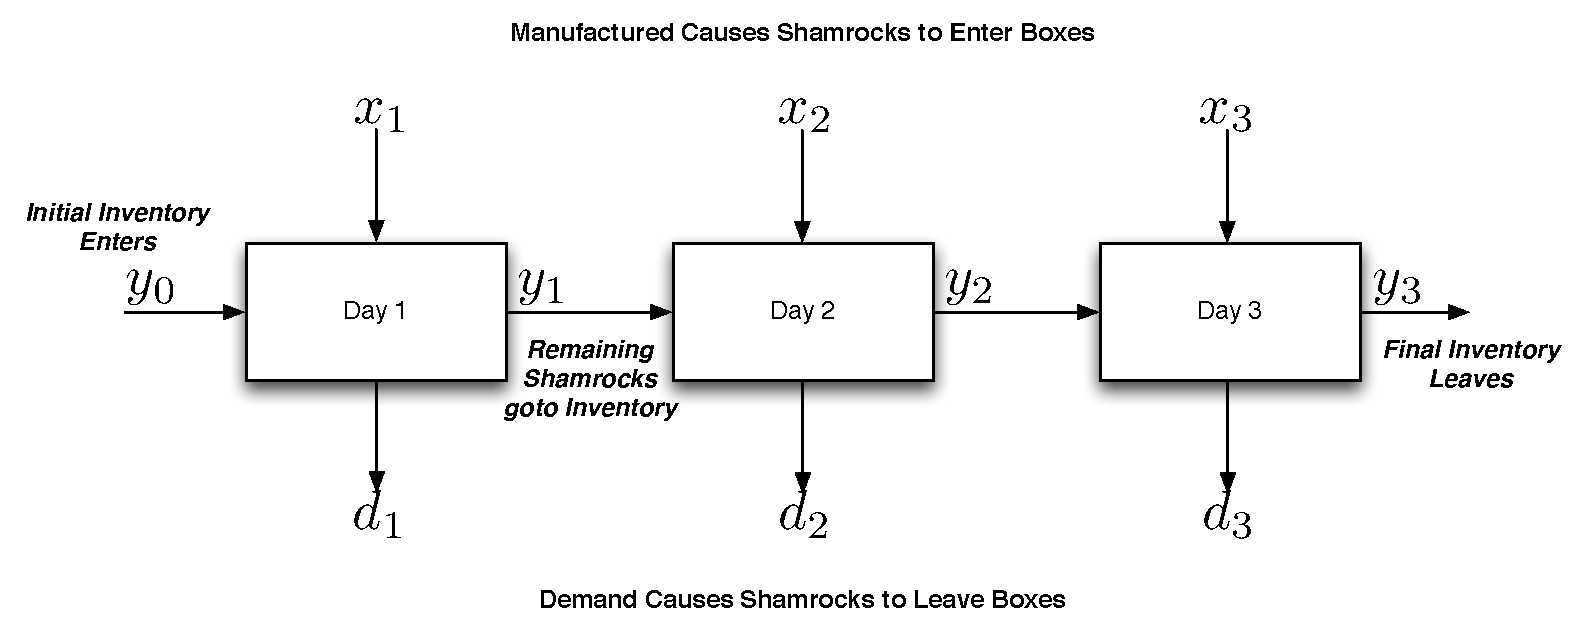
\includegraphics[scale=0.35]{ShamrockFigure.pdf}
\caption{Multiperiod inventory models operate on a principle of conservation of flow. Manufactured goods and previous period inventories flow into the box representing each period. Demand and next period inventories flow out of the box representing each period. This inflow and outflow must be equal to account for all production.}
\label{fig:Shamrock}
\end{figure}

This means that:
\begin{equation}
y_{t-1} + x_t = y_{t} + d_t\quad\forall t
\end{equation}
This equation says that at period $t$ the amount of inventory carried over from period $t-1$ plus amount of shamrocks produced in period $t$ must be equal to the total demand in period $t$ plus any left over shamrocks at the end of period $t$. Clearly we also know that $x_t \geq 0$ for all $t$, since you cannot make a negative number of shamrocks. However, by also requiring $y_t \geq 0$ for all $t$, then we assert that our inventory can never be negative. A \textit{negative inventory} is a \textit{backorder}. Thus by saying that $y_t \geq 0$ we are also satisfying the requirement that McLearey satisfy his demand in each period. Note, when $t = 1$, then $y_{t-1} = y_0$, which is the parameter we defined above.

The complete problem describing McLearey's situation is:
\begin{equation}
\left\{
\begin{aligned}
\min\;\;&200x_1 + 200x_2 + 200x_3 + y_1 + y_2 + 5y_3\\
s.t.\;\;&y_{t-1} + x_t = y_{t} + d_t\quad\forall t \in \{1,2,3\}\\
&x_t \leq 150\quad\forall t \in \{1,2,3\}\\
&x_t,y_t \geq 0\quad\forall t \in \{1,2,3\}
\end{aligned}\right.
\end{equation}
Constraints of the form $x_t \leq 150$ for all $t$ come from the fact that McLearey can produce at most 150 shamrocks per day.

This simple problem now has 6 variables and 6 constraints plus 6 non-negativity constraints and it is non-trivial to determine a good initial basic feasible solution, especially since the problem contains both equality and inequality constraints. 

A problem like this can be solved in Matlab (see Chapter \ref{chap:Matrices}.\ref{sec:Matlab}), or on a commercial or open source solver like the GNU Linear Programming Kit (GLPK, \url{http://www.gnu.org/software/glpk/}). In Figure \ref{fig:GLPKModel} we show an example \textit{model file} that describes the problem. In Figure \ref{fig:GLPKData}, we show the data section of the GLPK model file describing McLearey's problem. Finally, figure \ref{fig:GLPKOutput} shows a portion of the output generated by the GLPK solver \texttt{glpsol} using this model. Note that there is no inventory in Year 3 (because it is too expensive) even though it might be beneficial to McLearey to hold inventory for next year. This is because the problem has no information about any other time periods and so, in a sense, the \textit{end of the world} occurs immediately after period 3. This type of \textit{end of the world} phenomenon is common in multi-period problems.
\begin{figure}[htbp]
\scriptsize
\verbatiminput{Shamrock.mod}
\caption{Input model to GLPK describing McLearey's Problem}
\label{fig:GLPKModel}
\normalsize
\end{figure}

\begin{figure}[htbp]
\scriptsize
\verbatiminput{Shamrock.dat}
\caption{Input data to GLPK describing McLearey's Problem}
\label{fig:GLPKData}
\normalsize
\end{figure}

\begin{figure}[htbp]
\scriptsize
\verbatiminput{ShamrockOut.txt}
\caption{Output from \texttt{glpsol} on the McLearey Problem.}
\label{fig:GLPKOutput}
\normalsize
\end{figure}
\end{example}
